%% Los cap'itulos inician con \chapter{T'itulo}, estos aparecen numerados y
%% se incluyen en el 'indice general.
%%
%% Recuerda que aqu'i ya puedes escribir acentos como: 'a, 'e, 'i, etc.
%% La letra n con tilde es: 'n.


\chapter{Introducción}

A lo largo de la historia de la agricultura, el hombre ha desarrollado el mejoramiento vegetal en forma sistemática y lo ha convertido en un instrumento esencial para incrementar la producción agrícola en términos de cantidad, calidad y diversidad.  

El fitomejoramiento, en un sentido amplio, busca alterar la frecuencia alélica de los genes para obtener cultivares  genéticamente superiores, adaptados a condiciones específicas, con mayor rendimiento y mejor calidad que las variedades nativas o criollas \citep{Allard67}. En otras palabras, su objetivo es desarrollar genotipos cuya superioridad genética esté de acuerdo con las condiciones agroclimáticas donde se producen, necesidades y recursos de todos aquellos que producen, transforman y consumen productos vegetales. 

Las variedades mejoradas son el resultado del trabajo llevado a cabo en los programas de fitomejoramiento, los cuales se extienden por largo de varios años y requieren cuantiosas inversiones. Generalmente, en etapas tempranas de estos programas existe un gran número de genotipos experimentales con pocos antecedentes de evaluación; mientras que en etapas posteriores  se evalúan pocos genotipos que con más repeticiones y en más ambientes/años. Estos ensayos multiambientales (EMA) son herramientas fundamentales para evaluar la productividad para así asegurar la rentabilidad de los cultivos.

Como consecuencia de que los EMA se llevan a cabo en múltiples ambientes/años, la aparición de la interacción genotipo $\times$ ambiente (IGA) es inevitable debido a las variaciones en las condiciones climáticas y de suelo. La IGA es considerada por los fitomejoradores como el principal factor factor limitante de  respuesta a la selección y, en general, de la eficiencia de los programas de mejoramiento, por provocar respuestas altamente variables en los diferentes ambientes (\citet{Crossaetal1990}; Cruz Medina, 1992; Kang y Magari, 1996). Gauch y Zobel (1996) explicaron la importancia de IGA como: si no hubiera interacción, una sola variedad \ híbridos rendirían al máximo en todo el mundo, además los materiales podrían evaluarse en un solo lugar y proporcionarían resultados universales.


Peto (1982) ha distinguido las interacciones cuantitativas, conocida también como interacción sin cambio de rango o \emph{no crossover} (NCOI), de las interacciones cualitativas, denominada también con
cambio de rango o \emph{crossover} (COI) (Cornelius et al., 1996). Cuando dos genotipos X e Y tienen una respuesta diferencial en dos ambientes diferentes, y su ordenación permanece sin cambios, se dice que la IGA es del tipo NCOI (Figura \ref{fig:fig11}(A))\, es COI cuando hay cambios en el orden de los genotipos (Figura  \ref{fig:fig11}(B)), y. finalmente, es inexistente cuando los genotipos responden de manera similar en ambos ambientes (Figura \ref{fig:fig11}(C)). 


\begin{figure}[h]
\begin{center}
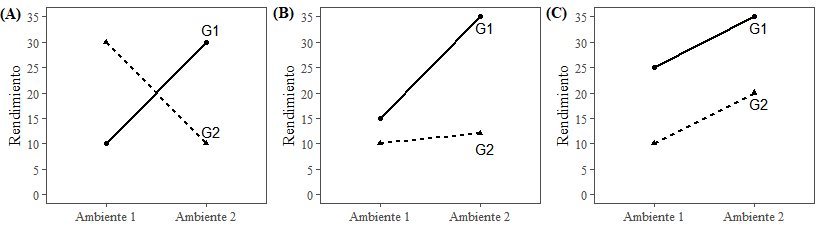
\includegraphics[width=14cm]{./Graficos/interac}
\end{center}
\caption{Representación gráfica de tipos de IGA: (A)IGA no crossover, (B) IGA crossover y (C) no IGA}
\label{fig:fig11}
\end{figure}


Entre las implicancias negativas de la IGA en los programas de mejoramiento se encuentra el impacto negativo sobre la heredabilidad, cuanto menor sea la heredabilidad de un caracter, mayor será la dificultad para mejorarlo. Como consecuencia, la información sobre la estructura y la naturaleza de la IGA es particularmente útil para determinar si se deben desarrollar cultivares con adaptación amplia o específica (Bridges, 1989). La decisión sobre qué tipo de estrategia seguir, involucra considerar y analizar  conceptos como regiones ecológicas, ecotipos y mega-ambientes (Kang et al., 2004).


La vigencia comercial de las variedades puede extenderse durante varias décadas, por lo que su elección es crítica para que el productor evite pérdidas económicas por malas campañas y el suministro al mercado sea constante. Consecuentemente, un análisis adecuado de la información de los EMA es indispensable para que el programa de mejoramiento genético de los cultivos sea eficaz. El rendimiento medio en los ambientes es un indicador suficiente del rendimiento genotípico solo en ausencia de IGA (Yan y Kang, 2003). Sin embargo, la aparición de IGA es inevitable y no basta con la comparación de las medias de los genotipos, sino que se debe recurrir a una metodología estadística más aporopiada. La metodología estadística más difundida para analizar los datos provenientes de EMA se basa en modificaciones de los modelos de regresión, análisis de variancia (ANOVA) y técnicas de análisis multivariado. 

Particularmente, para el estudio de la IGA y los análisis que de ella se derivan, dos modelos multiplicativos han aumentado su popularidad entre los fitomejoradores, especialmente como una herramienta de análisis gráfico: el modelo de los efectos principales aditivos e interacción multiplicativa (\emph{Additive Main effects and Multiplicative Interaction}, AMMI) (Kempton 1984, Gauch, 1988), y el de regresión por sitio (\emph{Site Regression model}, SREG) (Cornelius et al., 1996; \citet{GauchZobel1997} y 2002).  Estos modelos combinan un ANOVA con la descomposición de valores singulares (DVS) o un análisis de componentes principales (ACP) sobre la matriz residual de ANOVA. En SREG, el ANOVA se realiza sobre el eefecto principal o ambiental (A),  mientras que en AMMI el ANOVA se realiza sobre los efectos principales de genotipos (G) y A. Si bien a través del modelo AMMI se obtiene el gráfico biplot Genotipo $\times$ Ambiente (GA), el cual es usado para explorar patrones puramente atribuibles a los efectos la IGA, para el modelo SREG el biplot GGE es usado para explorar simultáneamente patrones de variación conjunta de G e IGA (Yan y Hunt (2002)).

Una limitación importante de la mayoría de las propuestas del análisis de EMA es que requieren que el conjunto de datos esté completo. Aunque los EMA están diseñados para que la totalidad de los genotipos se evalúen en todos los ambientes,  las tablas de datos genotipo $\times$ ambiente completas son poco frecuentes (no todos los genotipos se encuentran en todos los ambientes). Esto ocurre, por ejemplo, debido a errores de medición o pérdidas de plantas por presencia de animales, inundaciones o problemas durante la cosecha, además de la dinámica propia de la evaluaciones en las que se incorporan y se descartan genotipos debido a su pobre desempeño (Hill y Rosemberg, 1985). En estos casos, entre las posibles soluciones para tratar con una tabla de datos incompleta se encuentran: (i) el uso de un subconjunto completo de datos, eliminando aquellos genotipos que tienen valores faltantes (Ceccarelli et al., 2007, Yan et al., 2011), (ii) completar datos faltantes con la media ambiental, o (iii) imputar los datos faltantes con valores estimados utilizando modelos multiplicativos (Kumar et al., 2012). 



En este contexto, el análisis de datos provenientes de EMA requiere metodología estadística más sofisticada cuyas rutinas informáticas se encuentran disponibles en programas desarrollados por diferentes empresas. Esto genera el inconveniente de tener que disponer de todos los programas necesarios para los distintos análisis, atender los requerimientos de formatos de datos usados por cada uno de ellos, y comprender los diversos tipos de salidas en las que se ofrecen los resultados obtenidos. Además, algunos procedimientos, especialmente aquellas metodologías recientes, no se encuentran disponibles, y los costos de las licencias de dichos programas resultan muy elevados. 

Desarrollado por \emph{The R Foundation for Statistical Computing} el programa R se trata de un proyecto colaborativo de uso libre y distribuido bajo los términos de la \emph{General Public Licence} (GNU). R, surge como resultado de la implementación del lenguaje S uno de los más utilizados en investigación por la comunidad estadística. A diferencia de los programas estadísticos utilizados frecuentemente, R es un lenguaje de programación y no dispone de una interfaz gráfica que facilite el análisis usando menús, generando, su utilización, cierta dificultad para aquéllos que no se encuentran familiarizados con el lenguaje. Sin embargo,  por ser un software  libre,  permite a los usuarios definir sus propias funciones dando lugar a mayores posibilidades respecto del manejo y análisis de los datos disponibles. Si bien la versión básica del programa dista mucho de ser amigable, RStudio, un entorno de desarrollo integrado (IDE) gratuito y de código abierto para R, permite una interacción más fluida con el programa, actuando como una interfaz amigable con el usuario.  Al formar parte de un proyecto colaborativo, R promueve el hecho de que los usuarios compartan con la comunidad las funciones creadas por ellos, es decir que está en continuo desarrollo y actualización. A menudo, no resulta sencillo reutilizar una función creada por algún usuario, por ello, se ha introducido la posibilidad de crear paquetes (\emph{package}) o librerías. Éstas son una colección de objetos desarrollados y organizados siguiendo un protocolo fijo, lo cual garantiza un soporte mínimo para el usuario así como la ausencia de errores (de sintaxis) en la programación.

Actualmente, R cuenta con 14 paquetes básicos y 29 recomendados para su funcionamiento que se instalan automaticamente en él, tal como \emph{base} o \emph{stats}. Entre los paquetes que extienden las funciones básicas de R se encuentran, \emph{plyr}, \emph{lubridate}, \emph{reshape2} y \emph{stringr} para la manipulación de los datos; \emph{ggplot2} y \emph{rgl} para la visualización; \emph{knitr} y \emph{xtable} para la presentación de resultados; entre otros. La lista completa de los paquetes oficiales puede consultarse en CRAN\footnote{CRAN (Comprehensive R Archve Network) es el repositorio oficial de paquetes de R, el lugar donde se publican las nuevas versiones del programa, etc. Contiene la lista completa de paquetes oficiales. \url{https://cran.r-project.org/web/packages/available_packages_by_name.html}}, que contaba con más de 14.000 paquetes disponibles hasta junio de 2019. Esta gran variedad de paquetes es una de las razones de la gran difusión de R, ya que cada usuario puede tratar su problematica utilizando un paquete desarrollado por otro usuario. Además de los paquetes oficiales, existen otros que pueden instalarse desde repositorios como Github. Sin embargo, no es sencillo encontrar un paquete con todas las rutinas necesarias para el análisis, sino que debe recurrirse a varios de ellos. 

Con frecuencia, los mejoradores usan programas con interfaz gráfica para realizar el análisis estadístico, sin necesidad del manejo de un lenguaje de programación. En el año 2012 se creó el paquete \emph{Shiny} de R que facilita el desarrollo de aplicaciones Web utilizando R, acercando la potencia de R a todo tipo de usuarios, sin tener que programar.

El objetivo del presente trabajo es: (i) desarrollar un paquete de R para el análisis de datos provenientes de EMA que incluya metodologías existentes, modificadas para favorecer su uso, y otras recientemente publicadas y no disponibles en R y (ii) desarrollar una aplicación web Shiny que sirva como interfaz gráfica para el paquete sea más ágil de usar para aquellos que no tienen conocimientos del lenguaje de programación.
